
% Einleitung

\section{Elliptic Curve}
$y^2=x^3+a\cdot x+b \quad a,b,x,y \in \mathbb{R}$  $\to $ If an elliptic curve contains multiple roots, it cannot be used to form a group.\\
The negative of a point $P \equiv (x_p, y_p)$ is its reflection on the x-axis $\to$ $-P \equiv (x_p, -y_p)$.\\
Note: When in $\mathbb{F}_p$, all calculations are done with $\mod p$. Point at infinity $\mathcal{O}$ is additive identity of the elliptic curve group.

\subsection{Addition}
\begin{minipage}{12.5cm}
Add two Points on an Elliptic Curve. This is possible, if $4a^3+27b^2\neq0$
(Group patterns possible).\\
Geometric: 1. line through $P,Q \to$ intersection point $(-R)$. 2. Mirror on x-axes $\to R$.\\  

$m=\begin{cases}
\frac{3 \cdot x_p^2 + a}{2 \cdot y_P} & $ If $ P = Q\\
\frac{y_P-y_Q}{x_P-x_Q}               & $ If $ P \neq Q, P \neq -Q\\
\end{cases}$ 


$x_R = m^2 -x_p -x_q$ \\
$y_R = m(x_P-x_R)-y_p$\\
$\mathcal{O}+\mathcal{O}=\mathcal{O}, \quad P + \mathcal{O} = \mathcal{O} + P = P, \quad P+ (-P) = \mathcal{O}, \quad \mathcal{O}$: point at infinity.\\ 

\end{minipage}
\begin{minipage}{5.5cm}
  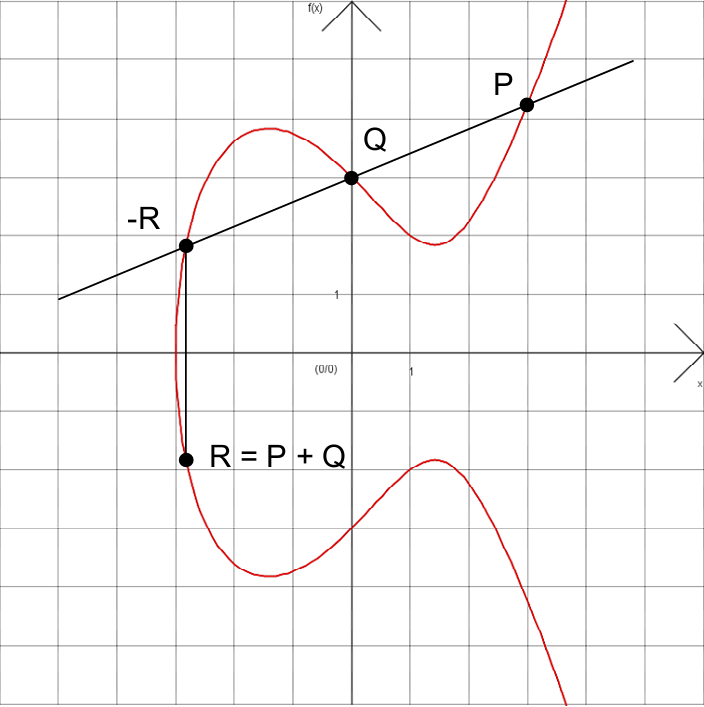
\includegraphics[width=5.5cm]{./bilder/elipticCurve.png}\\
\end{minipage} \\

\subsection{Number of Points and Order of a Point}
In cryptology elliptic curves with a high number of points are preferred.
Number of points on the elliptic curve $E(\mathbb{F}_p)$: $\#E(\mathbb{F}_p)=p+1-t$ with $|t| \leq 2 \cdot \sqrt{p}$ \\
For large $p$:  $\#E(\mathbb{F}_p) \approx p $ \\
For small $p$:  Calculate all the possible points of the curve and add $\mathcal{O}$.\\
\begin{minipage}{8cm}
	Example: $E: y^2=x^3-1$ over $\mathbb{F}_5$\\
	\begin{tabular}{|l |l|}
		\hline
		Possible values for $y$	&	Possible values for $x$\\
		\hline
		$0^2 \mod 5 = 0$		&	$0^3 - 1 \mod 5 = 4$\\
		\hline
		$1^2 \mod 5 = 1$		&	$1^3 - 1 \mod 5 = 0$\\
		\hline
		$2^2 \mod 5 = 4$		&	$2^3 - 1 \mod 5 = 2$\\
		\hline
		$3^2 \mod 5 = 4$		&	$3^3 - 1 \mod 5 = 1$\\
		\hline
		$4^2 \mod 5 = 1$		&	$4^3 - 1 \mod 5 = 3$\\
		\hline
	\end{tabular}
\end{minipage}
\begin{minipage}{10cm}
	As for the X-Values we got some results corresponding on the Y-side, we can combine them to evaluate the points of the curve: (0/2, (0/3), (1/0), (3/1), (3/4), $\mathcal{O}$.
	So, in total the given curve has 6 points.\\
\end{minipage}\\

The order of a point $P$ can be found by point multiplication: $n \cdot P=P+P+...+P$ for $n$ times $\to n$ is the smallest non-negative integer for which $n \cdot P=\mathcal{O}$. 
When calculating a new point, if $m\to \infty$ then the new point is at infinity, i.e. $\mathcal{O}$.\\

\subsection{Elliptic Curve Domain Parameters}
\begin{tabular}{l l p{11cm}}
	$T=(p,a,b,G,n,h)$	&	$p$		&	a prime $p$ specifying the finite field $\mathbb{F}_p$ \\
						&	$a,b$	&	two elements $a,b \in \mathbb{F}_p$ specifying an elliptic curve $E(\mathbb{F}_p)$ by the equation
										$E: y^2=x^3+ax+b \mod p$ \\
						&	$G$		&	a base point $G \equiv (x_g, y_g)$ on $E(\mathbb{F}_p)$\\
						&	$n$		&	$n$ which is the order of $G \to$ the smallest none-negative number $n$, for which $nG=\mathcal{O}$.\\
						&			&	order of Point always divides the total number of points.\\
						&	$h$		& 	$h$ is an integer which is the cofactor $h=\frac{ \#E(\mathbb{F}_p) }{n}$ \\
\end{tabular}\\

For cryptographic applications the order $n$ of $G$ must be a large prime with $\lceil \log_2(n) \rceil \geq 160$ (bit) and the cofactor $h$
should be a small number with $\lceil \log_2(h) \rceil \leq 10$ (bit).

\subsection{ECDH Elliptic curve Diffie-Hellman}

\begin{tabular}{l p{14cm}}
	1.	&	Alice and Bob agree upon a set of elliptic curve domain parameters $T=(p,a,b,G,n,h)$. \\
	2.	&	Alice randomly chooses a secret integer $d_A$ in the interval $[1,n-1]$ and computes $Q_A=d_A \cdot G$\\
	3.	&	Bob randomly chooses a secret integer $d_B$ in the interval $[1,n-1]$ and computes $Q_B=d_B \cdot G$\\
	4.	&	Alice and Bob exchange $Q_A$ and $Q_B$. The integers $d_A$ and $d_B$ are kept secret.\\
	5.	&	Alice computes $P_A=d_A \cdot Q_B$. Afterwards, $d_A$ can be deleted. \\
	6.	&	Bob computes $P_B=d_B \cdot Q_A$. Afterwards, $d_B$ can be deleted. \\
		&	\\
		&	The point $P_A$ and $P_B$ are equal, since $P_A=d_A \cdot Q_B = d_A \cdot d_B \cdot G = d_B \cdot Q_A = P_B \to P_A = P_B = P$.\\
		&	\\
	7.	&	If $P \neq \mathcal{O}$ then Alice and Bob take the x-coordinate $x_p$ as the shared key.
\end{tabular}

\subsection{ECDLP Elliptic Curve Discrete Logarithm Problem}

Given an elliptic curve $E(\mathbb{F}_p)$ over a finit field $\mathbb{F}_p$, a point $G$ on that curve and another point $Q$ you know to
be an integer multiple of $G$. The problem is to find the integer $n$ such $nG=Q$.\\
The security of elliptic curve cryptography rests on the assumption that the elliptic curve discrete logarithm problem is hard to solve.\\

\subsection{ECDSA Elliptic curve Digital Signature Algorithm}
We start with an elliptic curve $E(\mathbb{F}_p)$ over a finit field $\mathbb{F}_p$, a base point $G$ of order $n$.\\
To sign the message m, Alice does the following:\\
\begin{tabular}{l l}
	1. 	&	Select a random integer $k$ with $1 \leq k \leq n-1$. \\
	2. 	&	Compute $k \cdot G \equiv (x_1, y_1)$. \\
	3. 	&	Compute $r = x_1 \mod n$. If $r = 0$ then goto step 1.\\
	4. 	&	Compute $k^{-1} \mod n$.\\
	5. 	&	Compute $e = Hash(m)$.\\
	6. 	&	Compute $s=k^{-1} \cdot (e+d_A \cdot r) \mod n$. If $s = 0$ then goto step 1.\\
	7. 	&	Alice signature for the message $m$ is $(r, s)$.\\
\end{tabular}\\

To verify Alice's signature $(r, s)$, Bob must obtain an authentic copy of Alice domain parameters
and public key $Q_A$. Bob then does the following:\\
\begin{tabular}{l l}
	1. 	&	Verify that $r$ and $s$ are integers in the interval $[1, n-1]$.\\
	2. 	&	Compute $e = Hash(m)$.\\
	3. 	&	Compute $w = s-1 \mod n$.\\
	4. 	&	Compute $u_1 = e \cdot w \mod n$ and $u_2 = r \cdot w \mod n$.\\
	5. 	&	Compute $X = u_1 \cdot G + u_2 \cdot Q_A \equiv (x_1, y_1)$.\\
	6. 	&	If $X = \mathcal{O}$ then reject the signature. Otherwise compute $v = x_1 \mod n$.\\
	7. 	&	Accept the signature if and only if $v = r$.\\
\end{tabular}
